%iffalse
\let\negmedspace\undefined
\let\negthickspace\undefined
\documentclass[journal,12pt,twocolumn]{IEEEtran}
\usepackage{cite}
\usepackage{amsmath,amssymb,amsfonts,amsthm}
\usepackage{algorithmic}
\usepackage{graphicx}
\usepackage{textcomp}
\usepackage{xcolor}
\usepackage{txfonts}
\usepackage{listings}
\usepackage{enumitem}
\usepackage{mathtools}
\usepackage{gensymb}
\usepackage{comment}
\usepackage[breaklinks=true]{hyperref}
\usepackage{tkz-euclide} 
\usepackage{listings}
\usepackage{gvv}                                        
%\def\inputGnumericTable{}                                 
\usepackage[latin1]{inputenc}                                
\usepackage{color}                                            
\usepackage{array}                                            
\usepackage{longtable}                                       
\usepackage{calc}                                             
\usepackage{multirow}                                         
\usepackage{hhline}                                           
\usepackage{ifthen}                                           
\usepackage{lscape}
\usepackage{tabularx}
\usepackage{array}
\usepackage{float}


\newtheorem{theorem}{Theorem}[section]
\newtheorem{problem}{Problem}
\newtheorem{proposition}{Proposition}[section]
\newtheorem{lemma}{Lemma}[section]
\newtheorem{corollary}[theorem]{Corollary}
\newtheorem{example}{Example}[section]
\newtheorem{definition}[problem]{Definition}
\newcommand{\BEQA}{\begin{eqnarray}}
\newcommand{\EEQA}{\end{eqnarray}}
\newcommand{\define}{\stackrel{\triangle}{=}}
\theoremstyle{remark}
\newtheorem{rem}{Remark}
\begin{document}

\bibliographystyle{IEEEtran}
\vspace{3cm}

\title{Question 49, ME Gate 2023}
\author{EE23BTECH11017 - Eachempati Mihir Divyansh$^{*}$}
\maketitle
\newpage
\bigskip

\renewcommand{\thefigure}{\theenumi}
\renewcommand{\thetable}{\theenumi}
\textbf{Question:} Consider the second-order linear differential equation
\[x^2\frac{d^2y}{dx^2}+x\frac{dy}{dx}-y=0, \; x\geq 1\]
with the initial conditions $$y\brak{x=1}=6,\; \;\; \frac{dy}{dx}\big{|}_{x=1}=2.$$
Then the value of $y$ at $x=2$ is {\hfill(GATE ME 2023)}\\

\solution
%\fi
\begin{table}[h!]
    \centering
    \begin{tabular}{|m{2cm}|m{2cm}|m{2cm}|}
    \hline
    \textbf{Symbol} & \textbf{Value} & \textbf{Description}\\ [1ex]
    \hline
        $x$ & $x\brak{0}r^4$ & $x\brak{4}$ \\ [1ex]
    \hline
        $y$ & $x\brak{0}r^{10}$ & $x\brak{10}$\\ [1ex]
    \hline
        $z$ & $x\brak{0}r^{16}$ & $x\brak{16}$\\ [1ex]
    \hline
        $r$ & ? & $\frac{x\brak{n}}{x\brak{n-1}}$\\[1ex]
    \hline \vspace{0.1cm}
        $x\brak{0}$ & ? & First term \\[1ex]
    \hline
        $x\brak{n}$ & $x\brak{0}r^nu\brak{n}$ & General Term \\ [1ex]
    \hline
    \end{tabular}

    \caption{Given Information} \label{gateME49.tab:1}
\end{table}

% Consider the Mellin Transform
% \begin{align}
%     y\brak{x}\system{M}\int_{-\infty}^{\infty} x^{v-1}y\brak{x}{dx} 
% \end{align}
%  Let $$Y\brak{v}=\int_{-\infty}^{\infty} x^{v-1}y\brak{x}{dx} $$ 
%  Properties of the Mellin transform for a system at initial rest include 
% \begin{align}
%     y'\brak{x} &\system{M} -\brak{v-1}Y\brak{v-1}\\
%     xy'\brak{x} &\system{M} -v Y\brak{v}\\
%     \brak{x\frac{d}{dx}}^ny&\system{M} \brak{-v}^nY\brak{v} 
% \end{align}
% To modify this, evaluating the Mellin Transform specifically,
% \begin{align}
%     \brak{x\frac{dy}{dx}} &\system{M} \int_{-\infty}^{\infty} x^{v-1}\brak{x\frac{dy}{dx}}{dx}, \;\;x\geq1\\ 
%     &\system{M} \int_{1}^{\infty} x^{v}\brak{\frac{dy}{dx}}{dx}
% \end{align} 
% Integrating by parts, 
% \begin{align}
%     \brak{x\frac{dy}{dx}} &\system{M} [x^v\int \frac{dy}{dx}dx ]\big{|}_1 ^{\infty}-\int_1^{\infty} vx^{v-1}y\brak{x}dx\\
%     &\system{M} x^vy\brak{x}\big{|}_1^{\infty} -vY\brak{v}\\
%     &\system{M} \lim_{x\rightarrow{\infty}} \brak{x^v y\brak{x}}-y\brak{1}-vY\brak{v}
% \end{align} 
% Let \begin{align} L=\lim_{x\rightarrow{\infty}} \brak{x^v y\brak{x}} \label{gateME49.eq: 10}\end{align}
% Subject to $L=0$, from \eqref{gateME49.eq:24}, 
% \begin{align}
%     \brak{x\frac{dy}{dx}} &\system{M} -y\brak{1}-vY\brak{v}\\
%     \brak{x\frac{d}{dx}}^2 y &\system {M} v^2Y\brak{v}+vy\brak{1}-y'\brak{1}
% \end{align}
% The given differential equation can be written as: 
% \begin{align}
%     x\frac{d}{dx}\brak{x\frac{dy}{dx}}&=y,\;\;x\geq 1\\
%     \implies \brak{x\frac{d}{dx}}^2y&=y,\;\;x\geq 1
% \end{align}
% Taking Mellin transform on both sides, and from \eqref{gateME49.eq:27} 
% \begin{align}
%     v^2Y\brak{v}+vy\brak{1}-y'\brak{1}=Y\brak{v},\;\;v<-1
% \end{align}
% From \tabref{gateME49.tab:1}
% \begin{align}
%     Y\brak{v}&=v^2Y\brak{v}+6v-2\\
%     \implies Y\brak{v}&= \frac{6v-2}{1-v^2}\\&=-\frac{4}{v+1}-\frac{2}{v-1}
% \end{align}
% Mellin Inversion theorem
% \begin{align}
%     Y\brak{s} \system{M^{-1}} \frac{1}{2\pi j} \lim_{T \rightarrow \infty}\int_{a-jT}^{a+jT} x^vY\brak{v}dv
% \end{align}
% Here, there are 2 poles corresponding to $v=1$ and $v=-1$. The limits of integration indicate a contour that can be assumed to cover a plane on eiher side of the verical line $x=a$.
% \begin{align}
%     y\brak{x}=\frac{1}{2\pi j}\lim_{T\rightarrow \infty} \int_{1-jT}^{1+jT}x^v Y\brak{v}dv 
% \end{align}
% This can be thought of as a contour encompassing the plane on the left of $x=1$.
% Therefore
% \begin{align}
%     y\brak{x}=\frac{1}{2\pi j}\lim_{T\rightarrow \infty} \int_{1-jT}^{1+jT} \brak{-\frac{4x^v}{v+1}-\frac{2x^v}{v-1}}dv 
% \end{align}
% By Cauchy's Reidue Theorem
% \begin{align}
%     y\brak{x}&=-\frac{1}{0!}\lim_{v\rightarrow -1} \brak{v+1} \frac{4x^v}{v+1} - \frac{1}{0!}\lim_{v\rightarrow 1}\brak{v-1} \frac{2x^v}{v-1} \\
%     &= -\frac{4}{x} -2x
% \end{align}
% To find ROC of v, substituting y\brak{x} in \eqref{gateME49.eq: 10}
% \begin{align} 
%     &\lim_{x\rightarrow \infty} x^v \brak{-2x-\frac{4}{x}}=0\\ \label{gateME49.eq:24}
%     \implies& \lim_{x\rightarrow \infty} \brak{4x^{v-1}+2x^{v+1}}=0\\
%     \implies& \Re \brak{v+1}<0,\;\Re \brak{v-1}<0\\
%     \implies& \Re v<-1\label{gateME49.eq:27}
% \end{align}
By Euler-Cauchy substitution for the given question,
\begin{align}
    &x=e^t,\;\;t\geq 0 \label{gateME49.eqn:1}\\ 
    &\implies \frac{dt}{dx}=e^{-t}\\
    &\implies \frac{dy}{dx}=\frac{dy}{dt}\frac{dt}{dx}= e^{-t}\frac{dy}{dt}\\
    &\implies \frac{d^2y}{dx^2}=\frac{d^2y}{dt^2}\brak{\frac{dt}{dx}}^2+\frac{d^2t}{dx^2}\brak{\frac{dy}{dt}}\\
    &=e^{-2t}\frac{d^2y}{dt^2}+e^{-2t}\frac{dy}{dt} 
\end{align}
So the given equation becomes
\begin{align}
    &e^{2t}\brak{e^{-2t}\frac{d^2y}{dt^2}-e^{-2t}\frac{dy}{dt}} + e^{-t}\brak{e^{-t}\frac{dy}{dt}} -y=0\\
    &\frac{d^2y}{dt^2}-\frac{dy}{dt}+\frac{dy}{dt}-y=0\\
    &\frac{d^2y}{dt^2} - y=0,\;\;t\geq 0
\end{align}
Taking Laplace Transform, 
\begin{align}
    &s^2Y\brak{s}-sy\brak{0}-y'\brak{0}-Y\brak{s}=0\\
    &Y\brak{s}=\frac{sy\brak{0}+y'\brak{0}}{s^2-1}\\
    &=\frac{6s+2}{s^2-1}
\end{align}
By partial fractions,
\begin{align}
    Y\brak{s}=\frac{4}{s-1}+\frac{2}{s+1}
\end{align}
Taking Inverse Laplace using 
\begin{align}
    \frac{1}{s+a} \system{L^{-0}} e^{-at}
\end{align}
We get,
\begin{align}
    y\brak{t}=4e^{t}+2e^{-t}
\end{align}
From \eqref{gateME49.eqn:1}
\begin{align}
    &y\brak{t}=4x+\frac{2}{x}\\
    \implies &y\brak{2}=9
\end{align}
\begin{figure}[h]
    \centering
    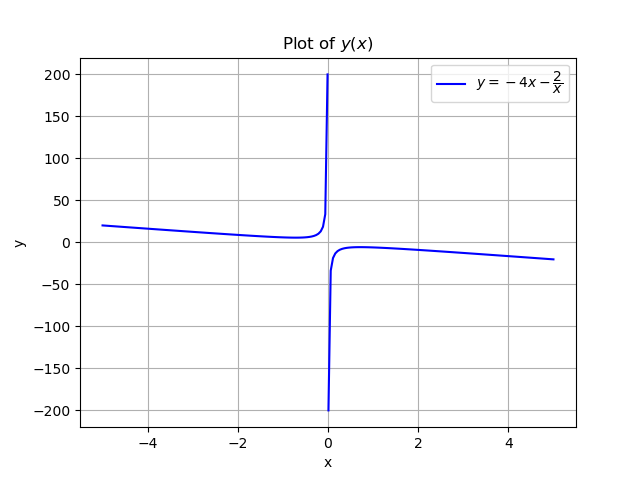
\includegraphics[width=\columnwidth]{figs/fig.png}
    \caption{Plot of $y\brak{x}$ v/s $x$}
\end{figure}

%\end{document}
